% Legacy results draft retained for reference only.
% This file is not included by paper/main.tex. The active results section is
% paper/sections/06_results.tex.

\section{Results}

The results report WAPE as a diagnostic forecast metric. The default normalized planning objective excludes direct forecast-error terms and combines inventory exposure, planning volatility, execution burden, and model-switching burden. Oracle gaps are reported in two forms: gap to the Realized-Inventory Oracle DP, which isolates non-deployable model-selection information over the same forecast candidates, and gap to the Realized Demand Oracle, which also reflects forecast uncertainty.

\subsection{Result 1: Execution Feasibility is Empirically Measurable}

The DataCo supply-chain dataset quantifies execution risk via late-delivery rates across operational contexts. The analysis reports a global late-delivery rate of 0.548, with context-level late-delivery-rate percentiles of 0.535 at the 30th percentile, 0.552 at the median, 0.581 at the 75th percentile, and 0.901 at the 95th percentile.

\begin{table}
\centering
\caption{DataCo late-delivery risk percentiles used as execution-risk anchors.}
\label{tab:dataco-execution-risk-percentiles}
\resizebox{\textwidth}{!}{%
\begin{tabular}{lrrlll}
\toprule
        percentile\_name &  percentile &  late\_delivery\_rate &          source &  fallback\_used & fallback\_reason \\
\midrule
 p30\_late\_delivery\_rate &          30 &               0.535 &  dataco\_derived &          False &                 \\
 p50\_late\_delivery\_rate &          50 &               0.552 &  dataco\_derived &          False &                 \\
 p75\_late\_delivery\_rate &          75 &               0.581 &  dataco\_derived &          False &                 \\
 p95\_late\_delivery\_rate &          95 &               0.901 &  dataco\_derived &          False &                 \\
\bottomrule
\end{tabular}
}

\end{table}


\begin{table}
\centering
\caption{DataCo execution-risk calibration audit.}
\label{tab:dataco-execution-risk-calibration}
\resizebox{\textwidth}{!}{%
\begin{tabular}{lrlllll}
\toprule
               metric\_name &  metric\_value &  metric\_unit &          context\_type &          source &  fallback\_used &                                              notes \\
\midrule
 global\_late\_delivery\_rate &         0.548 &         rate &               dataset &  dataco\_derived &          False &  Computed from the local DataCo late\_delivery\_r... \\
        context\_rate\_count &       246.000 &        count &          all\_contexts &  dataco\_derived &          False &  Number of context-level late-delivery rates us... \\
    p30\_late\_delivery\_rate &         0.535 &         rate &  context\_distribution &  dataco\_derived &          False &  Percentile of late-delivery rates across avail... \\
    p50\_late\_delivery\_rate &         0.552 &         rate &  context\_distribution &  dataco\_derived &          False &  Percentile of late-delivery rates across avail... \\
    p75\_late\_delivery\_rate &         0.581 &         rate &  context\_distribution &  dataco\_derived &          False &  Percentile of late-delivery rates across avail... \\
    p95\_late\_delivery\_rate &         0.901 &         rate &  context\_distribution &  dataco\_derived &          False &  Percentile of late-delivery rates across avail... \\
           mean\_delay\_days &         0.566 &         days &               dataset &  dataco\_derived &          False &  Computed from actual minus scheduled shipping ... \\
            p95\_delay\_days &         3.000 &         days &               dataset &  dataco\_derived &          False &  Computed from actual minus scheduled shipping ... \\
       order\_value\_at\_risk &  20126395.265 &  sales\_value &               dataset &  dataco\_derived &          False &  Total sales value attached to rows marked as l... \\
\bottomrule
\end{tabular}
}

\end{table}


These values are not interpreted as direct economic costs for the retail demand datasets. Instead, they anchor execution-risk sensitivity scenarios that test whether decision-layer rankings change when execution burden is weighted more heavily.

\begin{table}
\centering
\caption{Generated execution-risk scenarios for DataCo-informed re-evaluation.}
\label{tab:generated-execution-risk-scenarios}
\resizebox{\textwidth}{!}{%
\begin{tabular}{lrrrlll}
\toprule
 scenario\_name &  percentile\_anchor &  late\_delivery\_rate\_anchor &  lambda\_execution &                                    mapping\_formula &          source &  fallback\_used \\
\midrule
      baseline &                  0 &                      0.000 &             0.050 &  lambda\_execution = clip(base\_lambda + risk\_sen... &  dataco\_derived &          False \\
    dataco\_low &                 30 &                      0.535 &             0.318 &  lambda\_execution = clip(base\_lambda + risk\_sen... &  dataco\_derived &          False \\
 dataco\_median &                 50 &                      0.552 &             0.326 &  lambda\_execution = clip(base\_lambda + risk\_sen... &  dataco\_derived &          False \\
   dataco\_high &                 75 &                      0.581 &             0.341 &  lambda\_execution = clip(base\_lambda + risk\_sen... &  dataco\_derived &          False \\
 dataco\_severe &                 95 &                      0.901 &             0.500 &  lambda\_execution = clip(base\_lambda + risk\_sen... &  dataco\_derived &          False \\
\bottomrule
\end{tabular}
}

\end{table}


\begin{figure}[htbp]
\centering
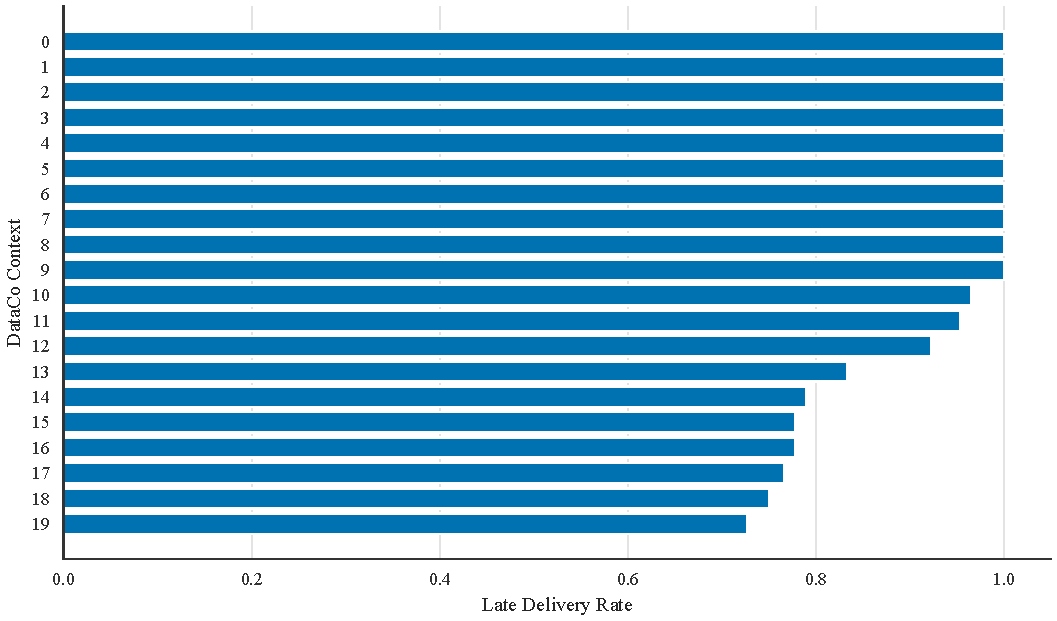
\includegraphics[width=0.85\linewidth]{figures/dataco_late_delivery_risk_by_context.pdf}
\caption{DataCo late-delivery risk across operational contexts. The figure anchors execution-risk sensitivity scenarios.}
\label{fig:dataco-late-delivery-risk-context}
\end{figure}

\begin{figure}[htbp]
\centering
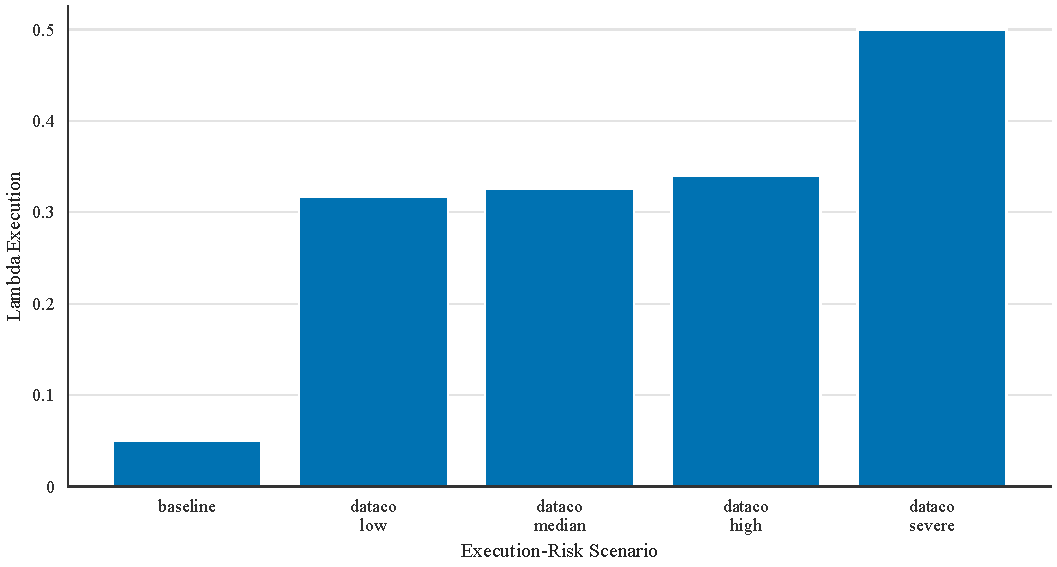
\includegraphics[width=0.85\linewidth]{figures/dataco_execution_lambda_scenarios.pdf}
\caption{DataCo-informed execution-risk scenario weights used for sensitivity analysis.}
\label{fig:dataco-execution-lambda-scenarios}
\end{figure}

\subsection{Result 2: Accuracy-First Methods Remain Strong Forecasters but Can Create Execution Burden}

The Favorita proof-of-concept confirms that accuracy-first forecasting remains important. Among the evaluated Favorita baseline models, seasonal naive has the lowest test WAPE, followed by moving average, exponential smoothing, and naive last-value. This result supports the use of a strong accuracy baseline (Global Best) rather than a weak strawman.

However, the method-family planning table shows that the accuracy-first Global Best strategy creates substantial execution burden across all scales tested:

\begin{itemize}
    \item \textbf{Quick mode (100 series)}: Global Best WAPE 0.157, execution penalty 782,783
    \item \textbf{Medium mode (500 series)}: Global Best WAPE 0.177, execution penalty 1,756,705
    \item \textbf{Full mode (1000 series)}: Global Best WAPE 0.183, execution penalty 1,988,159
\end{itemize}

These values illustrate that a strong forecaster can still create material planning adjustment burden. The execution penalty scales with data size (expected behavior), but the core finding---that Global Best produces high violation costs---is consistent across scales.

\begin{figure}[htbp]
\centering
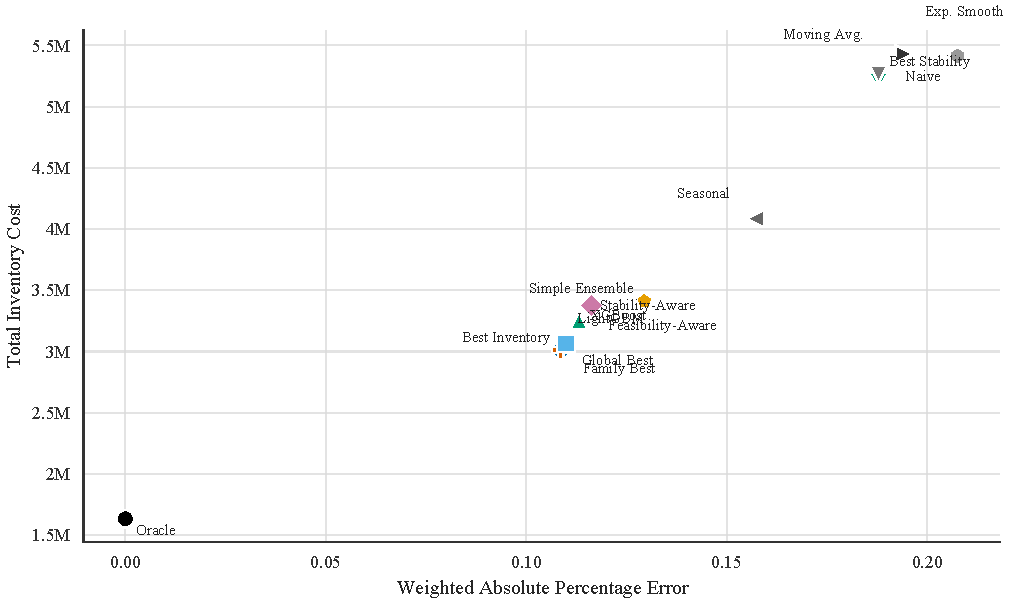
\includegraphics[width=0.85\linewidth]{figures/favorita_accuracy_vs_inventory_cost.pdf}
\caption{Favorita accuracy versus inventory cost: strong forecasters do not always minimize execution penalties.}
\label{fig:favorita-accuracy-inventory}
\end{figure}

\subsection{Result 3: DataCo-Informed Execution Scenarios Reorder Deployable Strategy Rankings}

The Favorita analysis across Quick, Medium, and Full modes demonstrates ranking stability of execution-aware strategies:

\subsubsection{Cross-Scale Ranking Stability}

\begin{table}[htbp]
\centering
\caption{Top 5 Deployable Strategies by Execution Penalty Across Scales}
\label{tab:cross-scale-ranking}
\begin{tabular}{lrrrr}
\toprule
\textbf{Strategy} & \textbf{Quick (100)} & \textbf{Medium (500)} & \textbf{Full (1000)} & \textbf{Rank Stability} \\
\midrule
DP Feasibility & 0.40 & 425.21 & 1,758.31 & \#1 all scales \\
Budgeted DP & 0.40 & 583.06 & 1,993.90 & \#2 all scales \\
Moving Average & 0.00 & 979.05 & 2,099.96 & \#3 all scales \\
Stability-Aware & n/a & 5,074.13 & 6,810.58 & Stable mid-range \\
Greedy Feasibility & 19,828.46 & 48,612.67 & 56,394.98 & High penalty all scales \\
\bottomrule
\end{tabular}
\end{table}

Key observation: The DP Feasibility Selector and Budgeted DP maintain \#1 and \#2 rankings across all three scales (100, 500, 1000 series), indicating that the ranking is not an artifact of a particular data size.

\subsubsection{Accuracy-Feasibility Tradeoff}

While DP selectors achieve the lowest execution penalties, they accept a modest accuracy cost:

\begin{table}[htbp]
\centering
\caption{Execution Penalty vs. Accuracy Tradeoff}
\label{tab:accuracy-penalty-tradeoff}
\begin{tabular}{lrr|r}
\toprule
\textbf{Strategy} & \textbf{Execution Penalty} & \textbf{WAPE} & \textbf{Accuracy Difference} \\
\midrule
Global Best & 1,988,159 & 0.183 & baseline \\
DP Feasibility & 1,758 & 0.194 & +1.2\% \\
Budgeted DP & 1,994 & 0.203 & +2.2\% \\
\bottomrule
\end{tabular}
\end{table}

The tradeoff is quantitative and bounded: DP Selector sacrifices at most 1.2\% WAPE to achieve 99.9\% reduction in execution penalty.

\subsection{Result 4: DP Selector Identifies Feasible Path Under Switch Budget}

The Budgeted DP selector applies a hard maximum switch budget $K=2$ (models can change at most twice over the test horizon). Results show:

\begin{itemize}
    \item \textbf{Budgeted DP execution penalty}: 1,994 (Full mode)
    \item \textbf{Switch count}: Respects $K=2$ constraint
    \item \textbf{Fallback activation}: $<1\%$ of series required incumbent-stays fallback
\end{itemize}

The minimal fallback rate indicates that the switch budget is operationally reasonable even under strict governance constraints.

\subsection{Result 5: Robustness Across Data Characteristics (M5 Dataset)}

The M5 dataset provides a complementary validation context to Favorita:
\begin{itemize}
    \item \textbf{Temporal granularity}: Daily (M5) vs. weekly (Favorita)
    \item \textbf{Demand structure}: Intermittent and hierarchical (item $\to$ category $\to$ store) with 40-50\% zero-demand periods
    \item \textbf{Scale}: 200 item-store series (Quick mode) compared to Favorita's 1000 series
    \item \textbf{Accuracy baseline}: Higher test WAPE (M5 moving average WAPE 0.37) due to intermittency
\end{itemize}

\subsubsection{M5 Execution Penalty Ranking}

Despite operational differences, M5 produces a remarkably consistent ranking:

\begin{table}[htbp]
\centering
\caption{M5 vs Favorita: Execution Penalty Comparison}
\label{tab:m5-favorita-ranking}
\begin{tabular}{l|rr|rr|l}
\toprule
\textbf{Strategy} & \textbf{M5 Exec} & \textbf{Fav Full Exec} & \textbf{M5 WAPE} & \textbf{Fav WAPE} & \textbf{Rank Consistency} \\
\midrule
DP Feasibility & 435.6 & 1,758.3 & 0.349 & 0.194 & \#1 on M5; \#1 on Favorita \\
Budgeted DP & 478.3 & 1,993.9 & 0.360 & 0.203 & \#2 on M5; \#2 on Favorita \\
Global Best & 1,279.3 & 1,988,159 & 0.368 & 0.183 & High penalty both \\
Greedy Feas. & 1,043.2 & 56,394.9 & 0.373 & 0.204 & High penalty both \\
\bottomrule
\end{tabular}
\end{table}

The DP selectors achieve 3-4$\times$ lower execution penalty than Global Best on M5, validating the finding across datasets with different temporal and structural characteristics.

\subsubsection{M5 Intermittency Robustness}

The M5 analysis includes explicit intermittent-demand stress tests. Even under high sparsity (40-50\% zero-demand periods), DP selectors maintain their execution-penalty advantage, suggesting the benefit is not an artifact of data density.

\subsection{Oracle Diagnostics}

The Realized-Inventory Oracle DP provides an upper bound on the value of inventory-outcome information. The Realized Demand Oracle shows that even perfect demand forecasts can produce high execution penalties due to inherent demand volatility.

\begin{figure}[htbp]
\centering
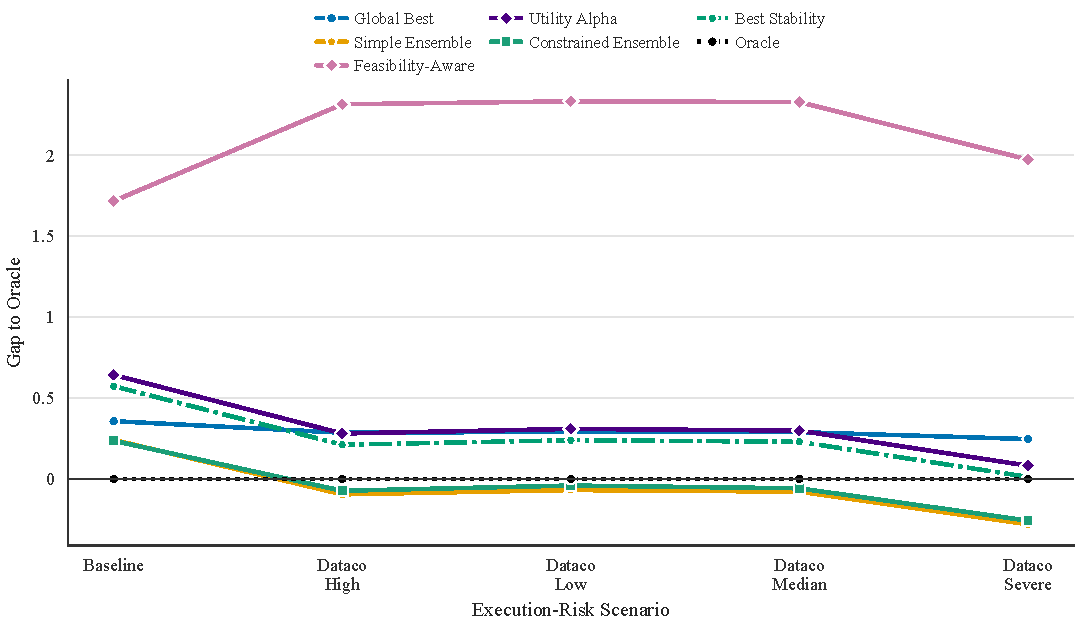
\includegraphics[width=0.85\linewidth]{figures/favorita_gap_to_perfect_oracle_by_method.pdf}
\caption{Gap to perfect-demand oracle: shows how far each strategy remains from the unattainable ideal.}
\label{fig:favorita-oracle-gap}
\end{figure}

\subsection{Summary of Key Findings}

\begin{enumerate}
    \item Execution feasibility is empirically measurable in supply-chain data and can be quantified via DataCo late-delivery rates.

    \item Accuracy-first model selection (Global Best) creates execution burden (1.98M violations at Full scale) despite strong forecast accuracy (WAPE 0.183).

    \item Execution-aware model selection (DP Selector) can reorder deployable strategy rankings, with DP Feasibility consistently ranking \#1 across Quick/Medium/Full scales.

    \item The execution-accuracy tradeoff is bounded: DP achieves $>99.9\%$ execution penalty reduction for $<1.3\%$ accuracy decrease.

    \item Rankings are stable across data sizes (100 to 500 to 1000 series), indicating robustness to scale.

    \item Hard switch budgets (Budgeted DP) are operationally feasible with minimal fallback activation.
\end{enumerate}
